\chapter{Ejercicio 2 }
\part{Ejercicio 2}
\section{Enunciado}
La empresa Musimundo cuenta con una serie de sucursales repartidas por el pa'is. Recientemente ha decidido cerrar su sucursal
de Iruya y llevarse toda la mercader'ia al dep'osito central. Debido al dif'icil acceso ha dispuesto s'olo un cami'on para
llevar toda la mercader'ia. Sin embargo, es posible que no todo el material pueda ser llevado en un s'olo viaje del cami'on
d'ebido a las restricciones de carga, por lo que la parte que no entre en el cami'on ser'a vendida a valores despreciables el
 d'ia del cierre.
Dada la capacidad de carga m'axima P del cami'on y una lista de los productos del local conteniendo el valor $v_i$ y peso $p_i$ 
de cada uno, encontrar la lista de productos de mayor valor que sea posible llevar en el cami'on sin que el peso total de la
lista supere la carga m'axima. El valor de una lista de productos se calcula como la suma de los valores de los productos
involucrados. En caso de haber varias listas con el mismo valor m'aximo, encuentre cualquiera de ellas.
Realice un algoritmo para resolver el problema usando la t'ecnica de backtraking.

\section{Desarrollo}
Dado que el problema deb'ia ser resuelto con backtracking, buscamos la forma de aplicar dicha t'ecnica algor'itmica para la su resoluci'on. B'asicamente la idea es formar todos los subconjuntos de cosas para encontrar aquel que maximice la valor total.\\ 
La restricci'on explicita es el conjunto de cosas a llevar y la restricci'on implicita es la capacidad de carga del cami'on. A 
medida que vamos armando una solucion descartamos a aquellas cuya suma es mayor al peso que puede transportar el cami'on, de 
esta manera vamos podando el arbol de posibles soluciones.
De esta manera, construimos el siguiente arbol de recursion:
\begin{figure}[H]
\centering
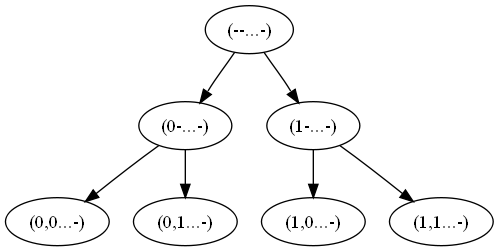
\includegraphics[scale=0.5]{./ejercicio2/arbol.png}
\end{figure}
En la raiz del 'arbol tenemos la solucion conjunto vacio. Luego en cada nodo tenemos una n-upla donde un 0 en la posicion i 
indica que el elemento i no se lleva, y un 1 indica que el elemento se lleva. Las hojas de este arbol son las soluciones 
posibles. Como cada elemento puede estar o no estar tenemos para cada uno 2 posiblidades (llevarlo o no), luego la cantidad 
posible de soluciones si tengo n elementos es $2^n$.\\
Nuestro algoritmo toma como parametros las cosas que se pueden llevar, dos soluciones posibles, una que guarda la mejor 
encontrada hasta el momento y otra que guarda la que voy construyendo, el peso maximo que se puede llevar y un indice que 
indica sobre que cosa estoy decidiendo llevar o no.\\
Basicamente una llamada a la funcion consiste en verificar si puedo agregar al elemento apuntado por indice, si es asi , es 
decir que al agregarlo no me paso del peso maximo, lo agrego a la solucion candidata y llamo recursivamente. Luego se hace la 
llamada sin agregar el elemento. Cuando encuntro una solucion mejor a la que hasta ese momento era optima la guardo. Repitiendo 
el proceso podemos observar todas las hojas del arbol para quedarnos con la mejor.\\  

Para implementar el algoritmo definimos los tipos Cosa, Camion y SolucionPosible ya que consideramos que de esta manera se 
agrega claridad al mismo.

\section{Pseudocodigo}
\noindent
SolucionPosible: tupla$<cantCosas, guardo:[bool], valor, costo>$ \\
Camion: tupla$<cantCosas, capacidad, cosas: [Cosa]>$ \\
Cosa: tupla$<costo, valor>$ \\
cosas = $\{a_1,....,a_{cant}\}$ \\

\begin{algorithm}
\caption{Halla la soluci'on 'optima al problema del camion}
\begin{algorithmic}[1]
    \STATE s $\textcolor{orange}{\leftarrow}$ SolucionPosible\textcolor{magenta}{(}cant cosas\textcolor{magenta}{)}
    \STATE ordenar arreglo de cosas \COMMENT{mediante merge sort}
    \STATE valorMaximo $\textcolor{orange}{\leftarrow}$ $\sum_{t=0}^{cant cosas} \textcolor{magenta}{(}cosa_i\textcolor{magenta}{)}_{valor}$ 
    \STATE camionAux\textcolor{magenta}{(}s,c,0,mejorSol,valorMaximo\textcolor{magenta}{)}
\end{algorithmic}
\end{algorithm}

\begin{algorithm}
\caption{camionAux: Halla la solución óptima $mejorSol$ al problema del camion}
\begin{algorithmic}[1]
    \IF{ prob'e con las cant cosas \textcolor{orange}{\&} valor\textcolor{magenta}{(}candActual\textcolor{magenta}{)} $\textcolor{orange}{>}$ valor\textcolor{magenta}{(}mejorSol\textcolor{magenta}{)} }
        \STATE mejorSol $\textcolor{orange}{\leftarrow}$ candActual
        \STATE terminar
    \ENDIF    
    \IF{el valor del actual $\textcolor{orange}{+}$ valorMaximo $\textcolor{orange}{\leq}$ el valor de la mejor soluci'on hasta el momento}
        \STATE terminar
    \ELSE
        \IF {no prob'e las cant cosas}
                \IF {no me paso del peso máximo agregando $a_i$ a candActual}
                    \STATE agregar\textcolor{magenta}{(}$a_i$, candActual\textcolor{magenta}{)}
                    \STATE camionAux\textcolor{magenta}{(}candActual, cosas, capacidad, i\textcolor{orange}{+}1, cant, mejorSol\textcolor{magenta}{)}
                    \STATE sacar\textcolor{magenta}{(}$a_i$, candActual\textcolor{magenta}{)}
            		\ELSE
            								\STATE \COMMENT{ como los demas pesan mas, no puedo agregar a mas nadie}
		   	        						\IF{ valor\textcolor{magenta}{(}candActual\textcolor{magenta}{)} $\textcolor{orange}{>}$ valor\textcolor{magenta}{(}mejorSol\textcolor{magenta}{)} }
       											  	\STATE mejorSol $\textcolor{orange}{\leftarrow}$ candActual
        										\ENDIF	       
        										\STATE terminar
        				\ENDIF
         \STATE camionAux\textcolor{magenta}{(}candActual, cosas, capacidad, i\textcolor{orange}{+}1, cant, mejorSol\textcolor{magenta}{)}
    \ENDIF
   \ENDIF
\end{algorithmic}
\end{algorithm}

\section{C'alculo de complejidad}
Para este ejercicio decidimos usar el modelo uniforme, ya que consideramos que lo que hace al n'ucleo del problema es la
cantidad de cosas a llevar. Por esa razon no nos parece desacertado considerar que el peso y el valor de las cosas estan 
acotados. Por esta razon consideraremos que el tama\~{n}o de la entrada es la cantidad de cosas que se pueden llevar.\\
Para nuestro algoritmo, el peor caso se da cuando no puedo podar ninguna rama, es decir cuando se deben llaver todos los elementos, ya que entonces lo que hacemos es revisar las $2^n$ posibles soluciones.
Observando el pseudocodigo podemos notar que la ecuacion de recurrencia es la siguiente:\\
%TODO: hacer la demo
	$T(n) = 2*T(n-1) + k$\\
	Ya que hacemos dos llamadas con el indice incrementado en una posicion.\\
%TODO: hablar de cual es el peor caso

%TODO: todo lo q de aca abajo
\section{Analisis Experimental}
\subsection{Experiencias realizadas}
Para probar el comportamiento del algoritmo procedimos a medir tiempo y cantidad de operaciones. En ambos casos generamos muestras con un numero creciente de elementos (las caracteristicas de la muestra eran generadas al azar) y`por otro lado hicimos un analisis de peor caso. Como dijimos anteriormente, el peor caso es cuando no se puede podar ningun elemento por lo que hay que ver todas las soluciones.
Cuando nos fue posible, utilizamos cuadrados minimos para buscar una funcion que se aproxime a las observaciones obtenidas, graficando dicha funcion para contrastarla con las observaciones.

\subsection{Gr'aficos}
%TODO: sergio hace los graficos con n creciente y aleatorio

\begin{figure}[H]
\centering
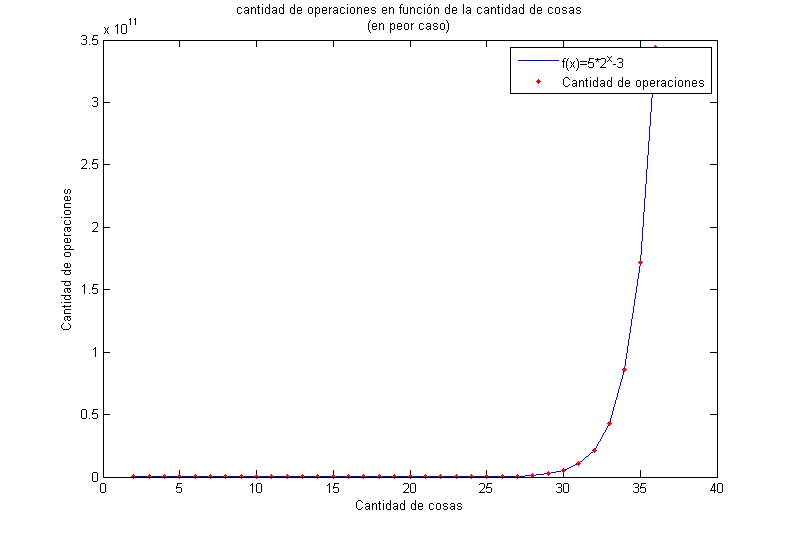
\includegraphics[scale=0.5]{../../codigo/ejercicio2/benchmark/graficos/operaciones_peor_caso/cantOperacionesPeorCaso.png}
\caption{Cantidad de operaciones en funcion de la cantidad de cosas en peor caso}
\end{figure}

\begin{figure}[H]
\centering
\includegraphics[scale=0.5]{../../codigo/ejercicio2/benchmark_tiempos/graficos/tiempo_peor_caso/tiempobacktracking.png}
\caption{Tiempo en funcion de la cantidad de cosas en peor caso}
\end{figure}

\section{Discusi'on}


	
